\documentclass{beamer}
\usepackage[utf8]{inputenc}

\usetheme{Madrid}
\usecolortheme{default}
\usepackage{amsmath,amssymb,amsfonts,amsthm}
\usepackage{txfonts}
\usepackage{tkz-euclide}
\usepackage{listings}
\usepackage{adjustbox}
\usepackage{array}
\usepackage{tabularx}
\usepackage{gvv}
\usepackage{lmodern}
\usepackage{circuitikz}
\usepackage{tikz}
\usepackage{graphicx}

\setbeamertemplate{page number in head/foot}[totalframenumber]

\usepackage{tcolorbox}
\tcbuselibrary{minted,breakable,xparse,skins}

\definecolor{bg}{gray}{0.95}
\DeclareTCBListing{mintedbox}{O{}m!O{}}{%
  breakable=true,
  listing engine=minted,
  listing only,
  minted language=#2,
  minted style=default,
  minted options={%
    linenos,
    gobble=0,
    breaklines=true,
    breakafter=,,
    fontsize=\small,
    numbersep=8pt,
    #1},
  boxsep=0pt,
  left skip=0pt,
  right skip=0pt,
  left=25pt,
  right=0pt,
  top=3pt,
  bottom=3pt,
  arc=5pt,
  leftrule=0pt,
  rightrule=0pt,
  bottomrule=2pt,
  toprule=2pt,
  colback=bg,
  colframe=orange!70,
  enhanced,
  overlay={%
    \begin{tcbclipinterior}
    \fill[orange!20!white] (frame.south west) rectangle ([xshift=20pt]frame.north west);
    \end{tcbclipinterior}},
}

\lstset{
    language=C,
    basicstyle=\ttfamily\small,
    keywordstyle=\color{blue},
    stringstyle=\color{orange},
    commentstyle=\color{green!60!black},
    numbers=left,
    numberstyle=\tiny\color{gray},
    breaklines=true,
    showstringspaces=false,
}

%------------------------------------------------------------
% Title info
\title{4.5.11}
\date{October 7, 2025}
\author{EE25BTECH11009 - Anshu Kumar Ram}

\begin{document}

\frame{\titlepage}

% Question
\begin{frame}{Question}
Find the cartesian equation of the line which passes through the point $(-2,4,-5)$
and parallel to the line 
\begin{align}
\frac{x+3}{3} = \frac{y-4}{5} = \frac{z+8}{6}
\end{align}
\end{frame}

% Solution (Vector Form)
\begin{frame}{Solution - Vector Form}
From the given line, the direction vector is
\begin{align}
\vec{m} = \myvec{3 \\ 5 \\ 6}
\end{align}

The required line passes through
\begin{align}
\vec{A} = \myvec{-2 \\ 4 \\ -5}
\end{align}

So, the vector equation is
\begin{align}
\vec{r} = \vec{A} + \lambda \vec{m}, \quad \lambda \in \mathbb{R}
\end{align}

In matrix form,
\begin{align}
\myvec{x \\ y \\ z} = \myvec{-2 \\ 4 \\ -5} + \lambda \myvec{3 \\ 5 \\ 6}
\end{align}
\end{frame}

% Solution - Cartesian Form
\begin{frame}{Solution - Cartesian Form}
Eliminating $\lambda$,
\begin{align}
\frac{x+2}{3} = \frac{y-4}{5} = \frac{z+5}{6}
\end{align}

Hence, the required cartesian equation of the line is
\begin{align}
\boxed{\;\frac{x+2}{3} = \frac{y-4}{5} = \frac{z+5}{6}\;}
\end{align}
\end{frame}

% Figure
\begin{frame}{Figure}
\centering
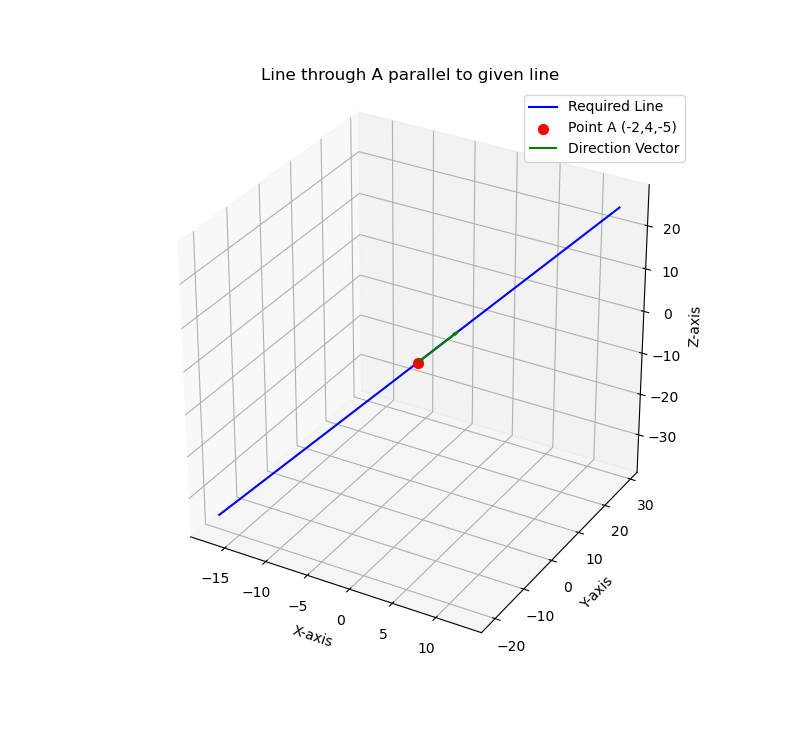
\includegraphics[height=0.5\textheight, keepaspectratio]{figs/Figure_1.png}
\end{frame}

\begin{frame}[fragile]{C Code - Part 1}
\begin{mintedbox}[fontsize=\scriptsize]{c}
#include <stdio.h>

// Function to fill point A
void get_point(int *A) {
    A[0] = -2; A[1] = 4; A[2] = -5;
}
\end{mintedbox}
\end{frame}

\begin{frame}[fragile]{C Code - Part 2}
\begin{mintedbox}[fontsize=\scriptsize]{c}
// Function to fill direction vector
void get_direction(int *m) {
    m[0] = 3; m[1] = 5; m[2] = 6;
}
\end{mintedbox}
\end{frame}

\begin{frame}[fragile]{Python + C Code - Setup}
\begin{mintedbox}[fontsize=\scriptsize]{python}
import numpy as np
import matplotlib.pyplot as plt
import ctypes

# Load the shared library
lib = ctypes.CDLL("./func.so")

# Create arrays for results
A = (ctypes.c_int * 3)()
m = (ctypes.c_int * 3)()

# Call C functions
lib.get_point(A)
lib.get_direction(m)

# Convert to numpy
point_A = np.array([A[i] for i in range(3)])
direction_vector = np.array([m[i] for i in range(3)])

print("Point A:", point_A)
print("Direction vector:", direction_vector)
\end{mintedbox}
\end{frame}

\begin{frame}[fragile]{Python + C Code - Parametric Line}
\begin{mintedbox}[fontsize=\scriptsize]{python}
# --- Generate line points using parametric form ---
lam = np.linspace(-5, 5, 100)
x = point_A[0] + lam * direction_vector[0]
y = point_A[1] + lam * direction_vector[1]
z = point_A[2] + lam * direction_vector[2]
\end{mintedbox}
\end{frame}

\begin{frame}[fragile]{Python + C Code - Plotting}
\begin{mintedbox}[fontsize=\scriptsize]{python}
fig = plt.figure(figsize=(8, 8))
ax = fig.add_subplot(111, projection='3d')

ax.plot(x, y, z, label="Required Line", color="blue")
ax.scatter(point_A[0], point_A[1], point_A[2],
           color="red", s=50, label="Point A (-2,4,-5)")
ax.quiver(point_A[0], point_A[1], point_A[2],
          direction_vector[0], direction_vector[1], direction_vector[2],
          color="green", label="Direction Vector", arrow_length_ratio=0.1)

ax.set_title("Line through A parallel to given line")
ax.set_xlabel("X-axis")
ax.set_ylabel("Y-axis")
ax.set_zlabel("Z-axis")
ax.legend()
ax.set_box_aspect([1,1,1])
plt.savefig("../figs/Figure_2.png")
plt.show()
\end{mintedbox}
\end{frame}

\begin{frame}[fragile]{Pure Python Code - Setup}
\begin{mintedbox}[fontsize=\scriptsize]{python}
import numpy as np
import matplotlib.pyplot as plt

# Required line: passes through A(-2,4,-5)
point_A = np.array([-2, 4, -5])

# Given line: passes through P(-3,4,-8)
point_P = np.array([-3, 4, -8])

# Direction vector (same for both lines)
direction_vector = np.array([3, 5, 6])

print(f"Point A (Required Line): {point_A}")
print(f"Point P (Given Line): {point_P}")
print(f"Direction Vector (m): {direction_vector}")


\end{mintedbox}
\end{frame}

\begin{frame}[fragile]{Pure Python Code - Plotting}
\begin{mintedbox}[fontsize=\scriptsize]{python}
# --- Parametric equations ---
lam = np.linspace(-5, 5, 100)
x_A = point_A[0] + lam * direction_vector[0]
y_A = point_A[1] + lam * direction_vector[1]
z_A = point_A[2] + lam * direction_vector[2]
x_P = point_P[0] + lam * direction_vector[0]
y_P = point_P[1] + lam * direction_vector[1]
z_P = point_P[2] + lam * direction_vector[2]
fig = plt.figure(figsize=(8, 8))

ax = fig.add_subplot(111, projection='3d')

# Plot the required line (Blue)
ax.plot(x_A, y_A, z_A, label='Required Line (through A)', color='blue')
ax.scatter(point_A[0], point_A[1], point_A[2],
           color='purple', s=50, label='Point A (-2,4,-5)')
ax.quiver(point_A[0], point_A[1], point_A[2],
          direction_vector[0], direction_vector[1], direction_vector[2],
          color='green', arrow_length_ratio=0.1, label='Direction Vector at A')
\end{mintedbox}
\end{frame}
\begin{frame}[fragile]{Pure Python Code - Plotting}
\begin{mintedbox}[fontsize=\scriptsize]{python}
# Plot the given line (Red dashed)
ax.plot(x_P, y_P, z_P, '--', label='Given Line (through P)', color='red')
ax.scatter(point_P[0], point_P[1], point_P[2],
           color='orange', s=50, label='Point P (-3,4,-8)')
ax.quiver(point_P[0], point_P[1], point_P[2],
          direction_vector[0], direction_vector[1], direction_vector[2],
          color='black', arrow_length_ratio=0.1, label='Direction Vector at P')

ax.set_title('Required Line and Given Line (Parallel)')
ax.set_xlabel('X-axis')
ax.set_ylabel('Y-axis')
ax.set_zlabel('Z-axis')
ax.legend()
ax.set_box_aspect([1,1,1])
plt.savefig("../figs/Figure_2.png")
plt.show()
\end{mintedbox}
\end{frame}
 \end{document}